\documentclass[a4paper]{jsarticle}
\usepackage{iapaper}
\usepackage[dvipdfmx]{graphicx}


\begin{document}
% 修士論文の場合は \degreethesis を使わず,下記を使う.
% なお博士の場合は \doctorthesisにすること
 \masterthesis
% 卒業論文の場合は下記を使う
% \degreethesis


\title{論 文 題 目}
\date{平成28年度}
\advisor{渡邉英徳} % 指導教員名を入れる
\IDnumber{15893507}
\Mauthor{木村汐里}% 自分の名前を入れる.修士の場合は \Mauthor{氏名} に変更する.
\submissiondate{平成29年1月25日}
\maketitle


\pagenumbering{roman} % 要旨はRoman書体で表示
\setcounter{page}{1} % 1から振り直す
\jasummary{論文タイトル}{副題(必要であれば記入)}\par
本研究では,集落組織が弱体化した過疎地域における「対話と交流の“場”」を形成する手法について検討する.そのために,新潟県魚沼市横根地区に実際に滞在し,住民とともに“場”の形成を実践していく.このことによって,弱体化した地域コミュニティーを強化することを企図している.\par
近年,地域活性化は国土政策における重要な課題となっており,国や自治体による政策・支援活動も数多く実施されている.しかし,トップダウンの財源と人的リソースは限られていることもあり,地域からの内発的な発展も強く求められている.その一方で,限界集落は地理的に不利な状況に置かれており,高齢化・人口減少などに伴って,集落組織の弱体化が急速に進んでいる.[1]従って,内発的な発展に必須な「地域コミュニティー」の力が弱まり,住民の地域主体性とシビックプライドが低下していることも,大きな課題となっている.これらを育む鍵となる「対話と交流の“場”」の形成についての先行事例は多数存在する.[2]しかし,過疎集落における地域活性化を目的とした例はない.\par
本研究ではこの点に着目し,地域主体性とシビックプライドを向上させる「対話と交流の“場”」を過疎集落において形成する手法について考察する.そのために,新潟県魚沼市横根地区の集落に実際に滞在し,地域住民とともに“場”の形成を実践する.\par
本論文は6章で構成される.\par
第1章では,本研究の概要,背景と研究目的について述べ,本論文の構成について説明する.\par
第2章では,先行研究を踏まえ,本研究における「地域活性化」の定義を「そこに住む人びとが地域の資源を活用し,生きいきとした創造的な生活を営んでいる状態,またはそうした目標に向かって努力している状態」と定める.さらに,限界集落における地域活性化の文脈における,本研究の位置付けを述べる.\par
第3章では,本研究で実践の場として横根地区を選定した理由を述べ,地域住民の地域関心を測るためにアンケート調査・現地調査を行い,それらの結果に基いて,対象地域の状況について詳述する.\par
第4章では,まず世古らの「参加と協働のデザイン」 [3]に基づき,平成26年度に対象地域で実施したワークショップについて検討し,「世代・性別を超えた交流が難しい」などの不満点を明らかにする.次いで,これらの不満点を解決するために,過疎地域の“場”の形成における設計・運営のガイドラインを定め,「パターン」にまとめる.\\
1)柔軟な枠組みに基づいた運営や進行\\
1-A:[目的におかない目標] :枠組みをもったアウトプット重視よりも対話や交流による創発性を通じた空間を重視する.\\
2)多様な世代が参加しやすいプロセス\\
2-A:[目線の多角化]:過疎地域の慣習上,“場”に参加しづらい世代に,参加に際して具体的な役割を付与する.\\
2-B:[伝達の最適化]:各世代に適した情報伝達の方法を用いて,“場”への参加を呼び掛ける.\\
3)参加者の想いや関心を自然に引き出す場づくり\\
3-A:[起爆のための仕込み]:事前に地域住民の意見を集め,フラットに表現するコンテンツを用意し,会話を促進する.\\
3-B:[協働作業]:様々な年代のメンバーが参加するチームを編成し,世代を超えた協働作業を行なう.\\
3-C:[自然体]:開催する場所・時間帯を,地域の慣習に合わせることにより,メンバーが気張らず,平常心で参加できるようにする.\par
 第5章では,第4章で設定した「パターン」を組み合わせて“場”を実践し,その有効性を検証する.どの年代でも気軽に参加できるクリスマス会をテーマに定め,地域住民の集会場である「みずほ会館」において“場”を形成する.子供たちには「地域へのプレゼント作り」を,若い世代の女性には「料理の準備」をそれぞれ,役割として担ってもらった.さらに8月の祭りにおけるインタビュー結果と,9月の小学校での地域発信ワークショップの結果をまとめ,“会話促進コンテンツ”を用意した.加えて,異世代のメンバーでチームを組み,クリスマスケーキを作ってもらった.こうした“場”を実践したところ,これまでの課題であった参加住民のばらつきが解消され,異世代・異性間における交流が促された.加えて“会話促進コンテンツ”により,地域に対する想いを語り合い,未来について深く議論する場面もみられた.これらの結果は,今回用いた「パターン」の組み合わせによって,適切な“場”が形成されたことを示している.従って,筆者の手法は有効なものであるといえる.さらに,自発的に地域行事を復活させようという声も上がった.この点は,本研究がもたらした効果が単年度に留まらず,継続していく可能性を示していると考えられる.\par
 第6章では,本研究の結論および研究成果が持つ意義を述べる.本研究で作成したパターンを組み合わせることで,地域主体性とシビックプライドを向上させる“場”を形成することができると言える.本研究の意義は,社会における重要な課題となりつつある「限界集落の地域活性化」のありかたについて,住民の地域主体性とシビックプライドの見地から再検討し,さらに実際の集落における「対話と交流の“場”」づくりの実践を通して,その有効性を示したことである.さらにこれらの“場”の形成を地域外に発信したところ,地域外からのフィードバックが地域内の地域愛着をあげている例もみられた.コミュニティーの強化が相互作用を生み,さらにはコミュニティーの拡張にもつながるといえる.本研究の成果は,専門家でなくとも利用可能であり,今後国内に増えていくと予想される限界集落における諸問題を解決するための,一つのモデルとなりうる.





\summary{Title}{Subtitle}
The author shall write a thesis in English text. 150 words.

\makemokuji


\newpage

\pagenumbering{arabic}  % 論文本体はArabicで表示
\setcounter{page}{1} % ページ番号を1から振り直す
\section{序論}
本研究の概要, 背景と研究目的について述べ,本論文の構成について説明する.
\subsection{本研究の概要}
本研究では,集落組織が弱体化した過疎地域における「対話と交流の“場”」を形成する手法について検討する.そのために,新潟県魚沼市の過疎地域である横根地区に実際に滞在し,住民とともに“場”の形成を実践する.
まず,先行研究や先行事例を整理し,限界集落における地域活性化の活動における「対話と交流の“場”」の位置付けを明らかにする. さらにワークショップ手法の先行事例について検討し,“場”における話題を促進するコンテンツと,世代・性別ごとの参加プロセスに注視することの重要性を導き出す.
この結論に基づき,過疎地域における「対話と交流の“場”」のプログラムデザインを設計する.実際の集落においてこのプログラムを用いて“場”の形成を実践を通して比較検証した結果,地域の多様な世代が参加し,活発な意見が交換される場が形成された.さらに,活動の内容をSNSで地域外に発信し,広く共有することによって,地域内外が相互作用を生む場も形成された.
このことから,創出したプログラムデザイン手法は妥当であり,過疎地域における対話と交流の“場”が形成を促されたといえる.これは,専門家でなくとも利用可能であり今後,国内に増えていくと予想される限界集落における諸問題を解決するための,一つのモデルとなりうる.
\subsection{背景と課題}
\subsubsection{地域活性化における内発的発展}
近年,地域活性化は国土政策における重要な課題となっており,なかでも,条件不利地域の維持に関する調査は,論点や調査方法こそ異なるが,各省庁によって(国土交通省\cite{1},)実施されている.このような現状に対して,まち・ひと・しごと創生本部や内閣府地方創生推進事務局の設置などを皮切りに,国土交通省重点政策\cite{2}の策定を始め,地域おこし協力隊の派遣など国や自治体による政策・支援活動も数多く実施されている.しかし,トップダウンの財源と人的リソースは限られていることもあり,依然として担い手の確保の状況は厳しく,地域からの内発的な発展が強く求められている.
\subsubsection{過疎地域における「地域コミュニティ問題」の現状}
過疎化とは,簡単にいうと地域の人口 (戸数)が急減し,そのことで産業の衰 退や生活環境の悪化がもたらされ,住民意識が低下し,最後には地域から人がいなくなる(集落が消滅する)ことと捉えられる.\cite{3}これは,農林水産業等の第一次産業から第二・三次産業へ の移行とそれに伴う農村部から都市部への人口移動という中で,すでに1960年代の高度経済成長期から「問題」として捉えられてきた.\cite{4}さらに山下は,「過疎問題」という 問題提起そのものが政治・行政によってなされ,財政的支援による中央との格差是正として解決が求められていくことで,結果として,過疎地域自身が問題を内発的に解決せずに, 地域はつねに政策の客体=受け手として振る舞うよう習慣化されてきたことを指摘している.\cite{5}
 さらに過疎地域の地域コミュニティでは,集落組織の弱体化が進んでおり,機会の減少や閉鎖的な空間であること,変化がおこりにくいなどの過疎集落の特徴がある.これらの特徴から地域の現在と未来に対して悲観的になり,集落機能や集落そのものの維持に対する関心を失い,それが結果として実際に集落機能や地域ネットワーク,集落そのものの喪失を早めるという,「負のスパイラル」ともいうべき現象が起きていると言われている.\cite{6}ゆえに,集落の人々が主体的に取り組む気持ちの涵養が重要視され,集落に居住していない人々,その地の出身者や近くの集落,また中心都市の人々を,集落に積極的に関わらせていく必要があると山下は論じている.\cite{7}


\subsection{本研究の目的}
筆者はこれまでに述べた背景を踏まえ,過疎地域の内発的な発展を推進するために必要不可欠である地域再生にむけた地域住民のモチベーションを高めるため,「対話と交流の場」を過疎集落において形成する手法について考察する.そこで以下のように目的と達成要件を定義した.
\begin{itemize}
\item 研究目的 \\「対話と交流の場」形成によって過疎地域における地域コミュニティーを強化する.

\item 達成用件\\過疎地域において「対話と交流の“場”」形成する手法について考察し,交流の“場”におけるガイドラインの設定を行う.

\end{itemize}

\subsection{本論文の構成}
本論文の構成を以下に示す.
\begin{enumerate}
\item 序論 … 本研究の概要,背景と研究目的・達成用件について述べ,本論文の構成について説明する.
\item 先行研究と概念の整理 … 先行研究と概念の整理を行い,限界集落における地域活性化活動での本論文の位置付けを述べる.

\item 対象地域… 本研究で実践の場として横根地区を選定した理由を述べ,地域住民の地域関心を図るためにアンケート調査・現地調査を行い,それらの結果から対象地域について詳述する.
\item 交流の“場”におけるガイドラインの設定 … 先行研究に基づき,ウェブサイト構築ワークショップについて検討し,「過疎地域の“場”の形成(手法)における設計・運営の指針を定め,「パターン」にまとめる.

\item 交流の“場”におけるガイドラインの有効性の検証…新潟県魚沼市横根集落において,第4章で設定した指針をもとに“場”の実践を行い,有効性の検証を行う.
\item まとめ…本研究の結論および研究成果が持つ意義を述べる.新たな問題点や展望をまとめる.


\end{enumerate}

\newpage

\section{先行研究と概念の整理}
本章では,地域活性化の定義をした後,地域活性化活動と地域住民の主体性・愛着との関係性を既存の研究から明らかにする.さらに過疎地域における地域活性化活動での本論文の位置付けを述べる.
\subsection{地域活性化とは}
地域活性化という言葉の意味には,「担い手形成」と「生産動向」に着目し,地域農林業の活性化状況(農林業活性化度)を捉えた「農林業活性化」や各市町村の「人口動態」と「人口構成」に着目した概念など,定義は様々ある.過疎地域において考えた場合,集落が人口減少にあるなかで,産業を生むことや,交流人口が単純に増やすことを考えるには破綻がある.そこで本研究では,塩見による,「活性化とはそこに住む人びとが地域の資源を活用し,生きいきとした創造的な生活を営んでいる状態,またはそうした目標に向かって努力している状態を指すのであろう」という提唱を活性化の定義とする.
 また,このような地域活性化を促す活動は,地域への愛着が強い人ほど居住継続意識を示し地域活動へ積極的に参加する意識が高いことや,町内活動やまちづくり活動などの活動に熱心であること\cite{8}がわかっている.地域に対する地域活性化活動はその土地に対する愛着やシビックプライドの醸成シビックプライドが高いことという二点が挙げられており,これを高めるためには住民の主体性や地域当事者性 (オーナーシップ) を育んでいくことが重要となる.

\subsection{対話と交流の“場”}
“場”に関して,清水博は,一般に人々が身体を関与させながら共創的コミュニケーションをおこなう 「共創の舞台」 を “場”と呼び\cite{9},伊丹敬之は,“場”とは,「人々がそこに参加し,意識・無意識のうちに相互に観察し,コミュニケーションを行い, 相互に理解し,相互に働きかけ合い,相互に心理的刺激をする,その状況の枠組みのこと」 「人々の間の情報的相互作用と心理的相互作用の容れもの」 と定義している\cite{10}. さらに,和田宰は,「異なる価値観や能力を持つ『ひと』」 が,相互作用を通じて創造的な活動を生み出していくためには,『創発』を生み出す相互作用の場をつくることが不可欠である」 「場が与えられることによって,それぞれの『ひと』は潜在的な価値観や能力を顕在化させ,他の『ひと』との相互作用を通じて,創造的な活動を生み出す可能性を得ることになる」 と“場”の重要性を指摘している\cite{11}.その上で,まちづくりの展開における“場”について,久隆浩は,地域に暮らす人々が集まり,自由に意見交換や情報交換し,楽しく気軽に話を展開し,その中から,気づきが生まれ,新たなつながりが生まれていく「交流の場」の重要性を指摘している\cite{12}これらの “場”の定義からもわかるように,地域活性化を促す活動においては,単に参加できる“場”の形成ではなく,対話や交流を通じて相互作用や関係変容が起こる “場”の形成が必要である. そうした“場”からつながりや輪が生まれ,活動や事業 (アクションやプログラム),組織が創発する. さらに,プロセスを通じてシビックプライド,市民の主体性や地域当事者性の育みが進み, 新しい公共の創出につながっていくことが期待される.\par“場”の形成手法については,ただ単純にひとが集まる“場”をつくれば,自動的に相互作用や関係変容が起こり,何かが生まれるというわけではなく,世田谷まちづくりセンターは,参加のデザインとして,①プロセスデザイン, ②プログラムデザイン,③参加形態のデザインの三つのデザインを挙げている[12].さらに世古一穂は,①参加のプロセスデザイン,②参加のプログラムデザイン,③参加構成のデザインの三つのデザインの重要性を挙げている.[13]状況に応じて,どのように場をデザインしていくのか,どのように運営していくのかという場づくりの方法が問われているといえる.このように“場”の形成手法については、多くの調査・研究がされてきたが、過疎集落における地域活性化を目的とした例はない.そこで本研究ではこの点に着目し,地域主体性とシビックプライドを向上させる「対話と交流の“場”」を過疎集落において形成する手法について考察する.






\section{対象地域}
本研究で実践の場として横根地区を選定した理由を述べ,アンケート調査・現地調査をもとに対象地域について詳述する.
\subsection{地域の概要}
本研究の対象地として、新潟県魚沼市横根地区を対象を選定した.筆者の所属する研究室が、平成26年7月より3月まで新潟県により大学生の力を活かした集落活性化事業の助成を受けている点、人口や高齢化率の規模が一般的な過疎地域と同等と言え本研究の対象に合致する点を考慮する.\parこの地区が位置する新潟県中越地方の南部に位置する魚沼市は、水や気候がコシヒカリの栽培に最も適していると言われ、米の名産地として知られている.2016年月現在の推計人口は約3万7千人である.\par魚沼市中心市街地から車で40分の場所に立地する横根地区は2016年4月現在の推計人口は121人、世帯数は56世帯、高齢化率50.4%の小規模山間地域である.日本海気象地区に属し、典型的な豪雪地帯であり、通年積雪3mにも及び、根雪日数は130日以上となっている.横根地区の地域資源としては、稲作があげられ、地域の7割以上の世帯が兼業ではあるが稲作を営んでいる.さらに市が運営する越後ハーブ香園入広瀬が集落の山頂に位置している.\par都市部からのアクセス条件は良いとは言えず、離村した若年層が頻繁に帰省できる距離でもない.古くから青年会、役員、老人会など、世代ごとの地域自治組織が存在していたが、人口の減少とともに形骸化し、現在は実質的にすべての自治組織の構成員と役割が同一化している.\par
 平成26年より総務省による地域力の創造・地方の再生の一環で地域おこし協力隊の派遣を受けている.


\begin{figure}[h]
  \begin{center}
    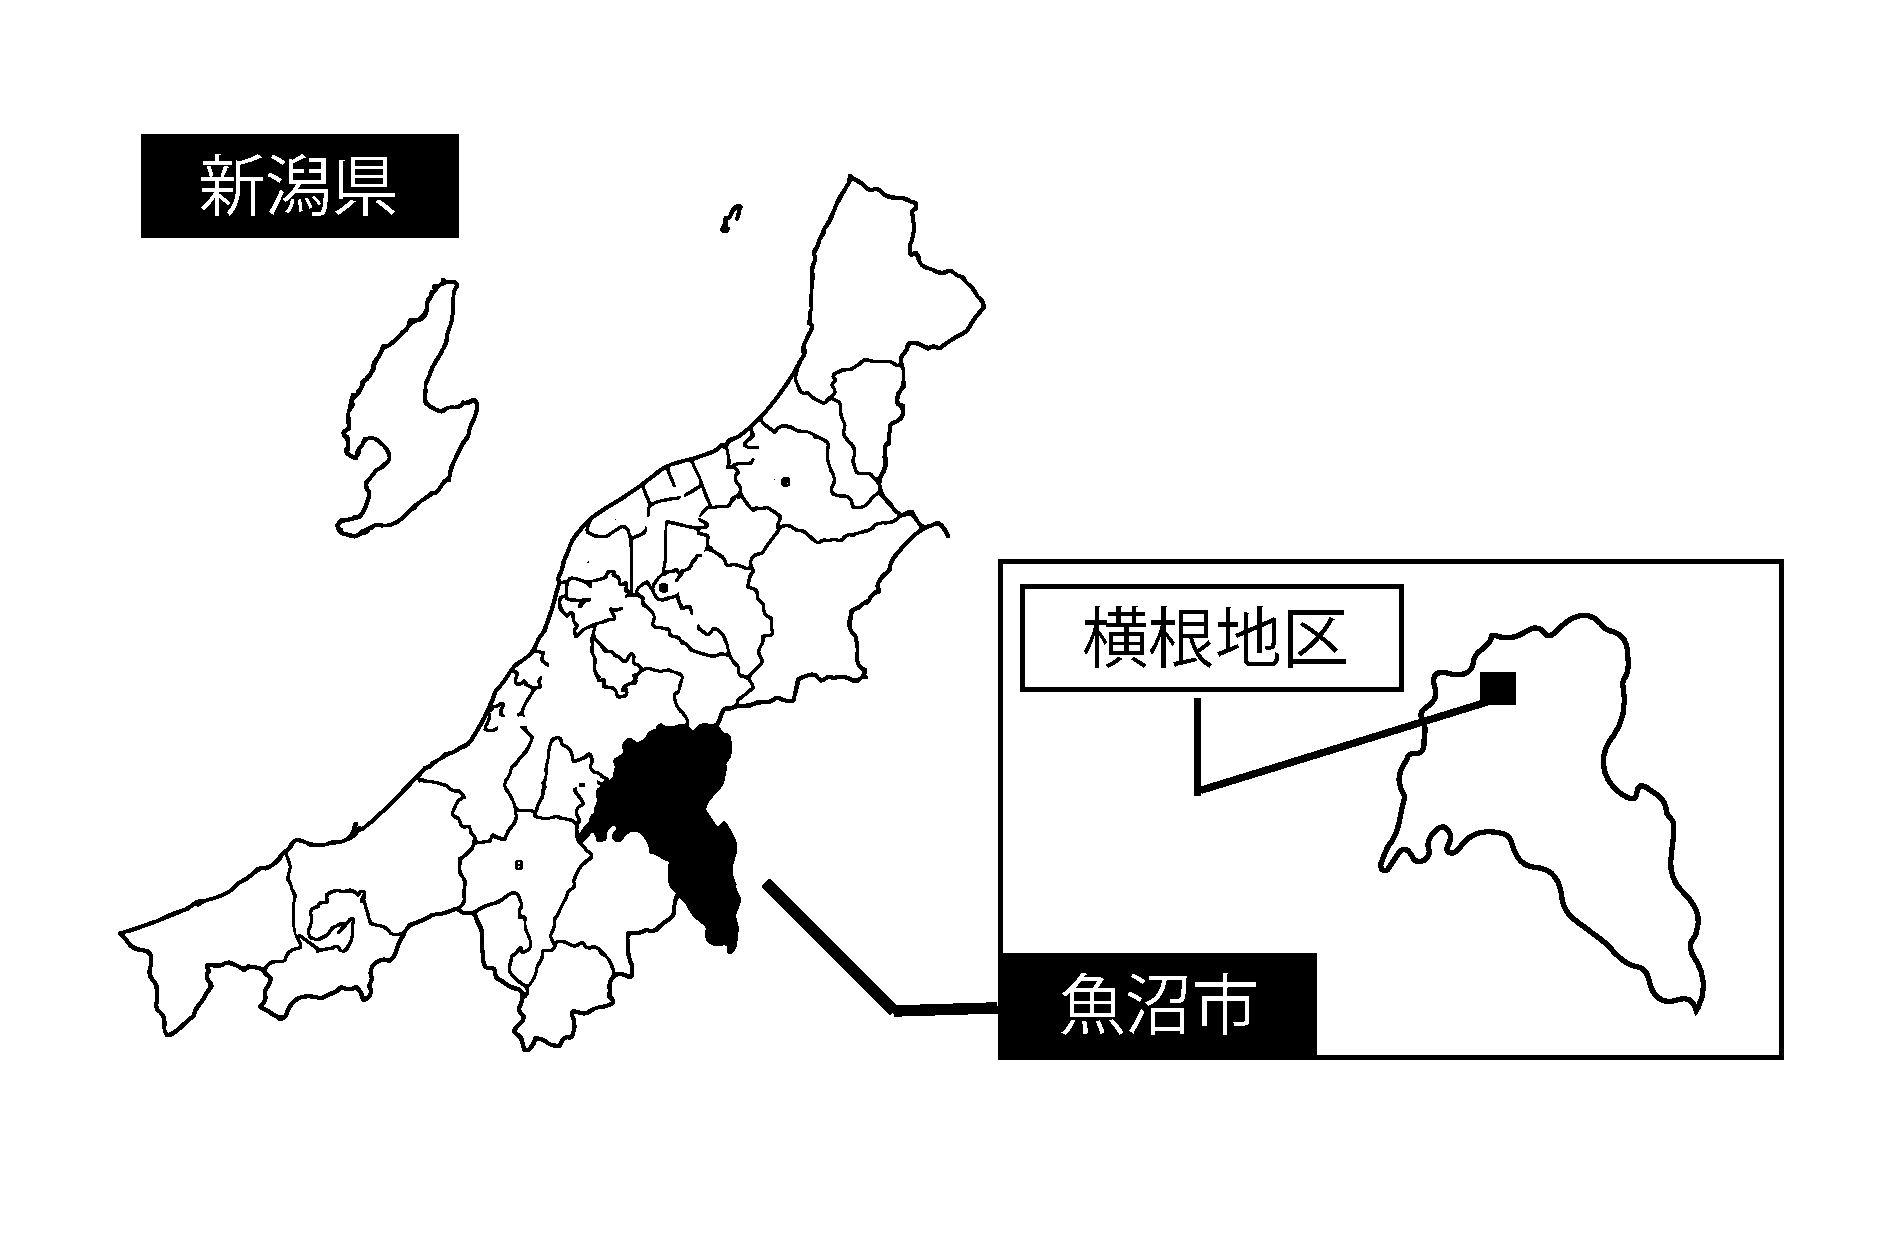
\includegraphics[width=0.95\hsize]{./images/yokone_place.pdf}
    \caption{魚沼市における横根集落の位置}
    \label{fig:tmu_hino}
  \end{center}
\end{figure}

\subsection{現地調査の実施}
横根地区の資料収集,地域資源の把握,現地住民への聞き取りなどを行うため,2014年7月31日〜8月2日、8月13日〜15日、2016年8月5日〜15日にて現地調査を行った.アンケート回収数は22,ヒアリングはおよそ20名に行った.\par

\begin{figure}[h]
  \begin{center}
    \includegraphics[width=0.95\hsize]{./images/02}
    \caption{アンケート調査1(地域への愛着意識調査)}
    \label{fig:tmu_hino}
  \end{center}
\end{figure}

住んでいる地域に対する評価として、「地域に対しての気持ちをおしえてください」の質問において、すごく嫌いーすごく好きまでの7段階評価で平均が5.8となり、自分の地域への愛着度が高いことがわかった。しかし、ヒアリングからは「こんなところにひとなんかこない。」「自分の生まれ育った地域だから愛着はあるけれど、できるなら出て行きたい。」などといった地域に対して後ろ向きな発言が多く聞かれ、シビックプライドが低いことがわかった。\par
\begin{figure}[h]
  \begin{center}
    \includegraphics[width=0.95\hsize]{./images/03}
    \caption{アンケート調査1(地域活性化に関する意識調査)}
    \label{fig:tmu_hino}
  \end{center}
\end{figure}

さらに地域の今後を考える地域活性化活動にについては、問題意識をもっているひとは大半を占めているにもかかわらず、自分で行動しようという主体性を持っている人は、全体の2割にも満たないことがわかった。\par地域には「役員会」と呼ばれる自治組織が存在しており,地域の決まりごとや大きな経費がかかるものに対して会議を行い、地域運営を行っていく10名ほどの集団が存在している。以前は他にも「子供会」、26歳~30歳の青年が集まり体育祭やレクリエーション,消防団の指導を行う「青年団」、花見や温泉旅行を行う「婦人会」、65歳になると入会する「老人会」などの年齢集団。さらに、消防練習を行う「消防団」や毎年行われる守門神社の祭りの運営を行う「祭り実行委員会」、農協や役場との農業の総括を行う「農業組合」などの機能集団が存在していたが、現在は人口の減少とともに形骸化し、現在は実質的にすべての自治組織の構成員と役割が同一化している。このため、世代ごとの連体感や世代を超えたコミュニケーションが減ってきている。\par地域のヒアリング調査からも、昔は毎年やっていた子供神輿などの地域行事や集まりが徐々に減少し、住民同士が世代・性別に関係なく集まる機会が減ってきているということがわかった.

\newpage
\section{交流の”場”におけるガイドラインの設定}
世古一穂らの「参加と協働のデザイン」\cite{10}に基づき,26年度に対象地域で実施したウェブサイト構築ワークショップについて検討し,不満点を解決するために,過疎地域の“場”の形成における設計・運営のガイドラインを定め,「パターン」にまとめる。
\subsection{ウェブサイト構築ワークショップ}
対話と交流の場づくりの一手法として「地域の問題を多くの住民がそれぞれの年齢や社会的な立場にとらわれることなく, 水平的な関係で話し合い, 創造的自己解決していくための場」\cite{10}として「ワークショップ手法」が様々な場面で広く使われ, 具体的な成果も出ている. その点から,平成26年に対象地域で菊本\cite{10}を中心に行ったウェブサイト構築ワークショップを対話と交流の”場”づくりの観点から考察する.
\subsubsection{概要}
2014年10月12日、横根集落内にあるみずほ会館において、地域の魅力を発信するWEBアプリ作成のためのマッピングワークショップを行った。参加者は集落在住の50~70代の男性9名、女性1名 計10名となった。運営は研究室メンバー6名、外部協力者1名の計6名で行った。紙地図を使用した作業と、ウェブ構築作業の二部構成でおこなった。手順は以下の通りである。なお、告知時に参加者には横根集落で撮影された写真を持参するように依頼している。\\

\item 1 … 事前に制作したデモ版を元にした最終イメージの共有。
\item 2 … 集落の地図を1.5[m]×2[m]の紙地図に印刷し、それを囲みながら持参した写真の撮影場所、撮影時期、当時の状況を話しあう。


\item 3… 特定されたら、紙地図上の撮影場所に写真をマスキングテープで貼付する。また、時期や状況はポストイットに記入し、写真に貼付する。

\item 4 … データ作成の担当を決定する。

\item 5…マッピングシステムを利用し、写真データに位置情報、撮影年代、撮影者,状況などを付与する。
\item 6…成果物観覧
\subsection{考察}
世古一穂らの「参加と協働のデザイン」より、1)場の運営、2)個々の場の位置づけ, 3)場の設計の三点から、ワークショップを検討する。\\\\
\item 1)場の運営\\
テーマを、『地域のアーカイブをつくるための制作体験講習会』とし、紙地図を使用した作業と、ウェブ構築作業の二部構成で行った.場づくりにおいて何らかの意思・意図があるが, 「ファシリテーション」 を通じて特定のゴールに誘導していくものではなく, 状況に対して, しなやかで, かつ, 柔軟に対応していくことが求められているが, 地域活動に対して意欲がある人が集まっているわけではない過疎集落の状況で今回の制作物が決まっている講習会形式でテーマ設定を行うと,  プロセスを通じて方向性・枠組み, 目的・目標自身が変化していくことに柔軟に対応することが難しく、「やらされている感」「よくわからない感」を感じている参加者がでてきてしまい、当事者意識の醸造にはハードルが高いことがわかった。あらかじめ明確な目標を設定した上で話し合いを行うことよりは, 対話や交流を通じてアクションが創出されることを期待した場づくりが有効であると考えられる。\\

\item 2)個々の場の位置づけ\\
地域内でのワークショップの告知は,普段から情報伝達に使われている地域の回覧板にチラシを挟む形で行った.(図4)その結果,参加したほとんどの住民が50-70代の男性であり、全員当時の地域自治組織の構成員であることがわかった.普段から, 共同体意識が強く,“決まりであるから”,“集落のためになるから”という理由で集まりに参加する意識があるという.その一方で,地域に古くからある地域行事の中心は家長である男性が代表となって行うという慣習から,女性が地域活動に積極的に参加しにくいということが分かった.地域には出身者であり、一度集落を出たが、戻ってきた若い母親が何人かいるが,地域活動にはあまり前向きではなく、「男の人がいくもの」「自分たちのでる幕でない」といおもっていることがヒアリングから聞こえてきた.全体の枠組みから見て個々の場の位置づけがどのような視点であるのかを明確にしておく必要がある.\\
\begin{figure}[h]
  \begin{center}
    \includegraphics[width=0.95\hsize]{./images/03}
    \caption{アンケート調査1(地域活性化に関する意識調査)}
    \label{fig:tmu_hino}
  \end{center}
\end{figure}

\item 3)場の設計\\
テーマを、『地域のアーカイブをつくるための制作体験講習会』とし、紙地図を使用した作業と、ウェブ構築作業の二部構成で行った.久隆によると、交流の場の運用上の課題として, 参加者の主体性・自発性・自律性によって活動が展開されること, 他者に対して活動を強制しないこと, 個人の資格で参加すること, 多様な主体が参加することを挙げている。\cite{10}紙地図作業では,「この写真は〇〇にきけばわかるかな」「〇〇さんならくわしいかもしれない」などと自発的に写真や地図を介して地域住民同士でのコミュニケーションが多く取られているのをみることができた. (図5)さらに学生のスタッフに対しては、「この時代はこんなだったんだよ」と、当時の状況を詳しく話す場面も見られた. (図6)その一方でウェブ構築作業については,「難しい」「わからない」などの意見が多く聞かれ、全ての作業工程をスクリーンショットと説明とともにおさめた手順書やマッピングシステムなどを作成して、参加者のハードルをさげようと試みたが,技術のハードルが参加者の主体性を削いでしまっている点が課題として見えた。その後のヒアリングで自分が制作に携わったという当事者意識は芽生えておらず,「なんかむずかしかった」「よくわからない」などという意見が多かった.
多様な主体という点においても,参加者は地域自治をになる50代から70代の男性がほとんどである点から課題があげられる.参加者を多様な世代にする、かつその様々な世代が自然と交流できる“場”を意識する必要があると考えられる.\\\\\\\par

\begin{figure}[h]
  \begin{center}
    \includegraphics[width=0.95\hsize]{./images/03}
    \caption{アンケート調査1(地域活性化に関する意識調査)}
    \label{fig:tmu_hino}
  \end{center}
\end{figure}
\begin{figure}[h]
  \begin{center}
    \includegraphics[width=0.95\hsize]{./images/03}
    \caption{アンケート調査1(地域活性化に関する意識調査)}
    \label{fig:tmu_hino}
  \end{center}
\end{figure}


これらの検討から、過疎地域の“場”の形成における大きな課題として「参加者の世代・性別のばらつき」、当事者意識の低い地域住民に対する「地域活動へのハードル」があげられることがわかった.



\subsection{過疎地域における交流の”場”におけるガイドライン}

これらの課題を解決するために,1)場の運営、2)個々の場の位置づけ, 3)場の設計の枠組みにおいて、過疎地域の“場”の形成における設計・運営のガイドラインを定め,「パターン」にまとめる。\\\\

\item 1)場の運営…『場の運営柔軟な枠組みに基づいた運営や進行』\\
1-A:[目的におかない目標] :枠組みをもったアウトプット重視よりも対話や交流による創発性を通じた空間を重視する.\\\\
地域活動を目的にした“場”の形成において,最終的に評価されるのは「結果」であるため、それを生み出す「プロセス」には目が行きにくく、継続性や当事者性が低い
成果物や意思決定が生まれてしまいがちである.そこでまずは地域活動を目的におかず、目標として捉え対話や交流を通じた相互作用や関係変容を大事にする. プログラムはあるが, 必ずしもプログラム通りに実施するのではなく, 状況に応じた柔らかなマネジメントを心がける. フレーム (枠組み) も状況に応じて,再構成し, ゴール自身も変化させる. さらに話し合いが単に楽しかっただけに留まらず, 次に前向きな展開になるように心がけるようにする.\\\\

\item 2)個々の場の位置づけ…『多様な世代が参加しやすいプロセス』\\
2-A:[目線の多角化]:過疎地域の慣習上,“場”に参加しづらい世代に,参加に際して具体的な役割を付与する.\\\\
過疎地域の地域住民はそれぞれ違うことに関心を持っており, 地域活動への関わり方も異なる. 特に当事者意識が低い世代に対して,まず参加してもらうことが第一の課題である.そこで,まずは地域活動の文脈に限らず世代ごとにその世代にあった“場”における役割を担ってもらうことで参加のハードルを下げるようにする.一つの“場”っであっても様々な目線があることを意識する.\\\\

2-B:[伝達の最適化]:各世代に適した情報伝達の方法を用いて,“場”への参加を呼び掛ける.\\\\
従来おこなわれている回覧板での情報伝達だけではなく,各世代に適した情報伝達の方法を使い分けるようににする.世代ごとの呼びかけ方も考慮する.\\\\


\item 3)場の設計…『参加者の想いや関心を自然に引き出す場づくり』\\
3-A:[起爆のための仕込み]:事前に地域住民の意見を集め,フラットに表現するコンテンツを用意し,会話を促進する.\\\\

人口の減少とともに対話や交流が減ってきた過疎地域において,自発的に地域活性のための対話や交流が生まれることは難しい.そこでWEBアプリ作成のためのマッピングワークショップの写真を使った紙地図作業を参考にし,会話を促すための起爆剤となるコンテンツを用意する.参加者が身近に感じられるように,地域関係者が関係した資料を収集する.\\\\

3-B:[協働作業]:様々な年代のメンバーが参加するチームを編成し,世代を超えた協働作業を行なう.\\\\
ただ“場”を用意したところで,同じ世代や親戚、関わりが多くある人とばかり話がちになってしまう.普段関わることの少ない世代や性別同士をあえて混ぜたグループを作り、協働作業を行うことでより新しい相互作用や関係変容が期待できる.\\\\
3-C:[自然体]:開催する場所・時間帯を,地域の慣習に合わせることにより,メンバーが気張らず,平常心で参加できるようにする.\\\\
改めて“場”ということを意識し強調してしまうと,縮こまり緊張してしまい,会話が弾まない.フラットな関係性でお互いが自然体で参加できるように地域の慣習をヒアリングし“場”の設計を考慮する.

\\\\

\newpage
\section{交流の”場”作りにおけるガイドラインの検証}
新潟県魚沼し横根集落において、本研究で設定したガイドラインの軸に作成した幾つかのパターンを元に今回の”場”作りを実践・考察し、ガイドラインの有効性の検証を行う.

\subsection{概要}
2015年12月12日横根集落内にあるみずほ会館において、どの年代でも気軽に参加できるクリスマス会”をテーマに定め,ガイドラインに沿って、“場”の形成を行う.話題促進コンテンツは、事前にお祭りでのインタビュー,小学校でのワークショップを行い,用意する.参加者は集落在住の50~70代の男性7名と女性4名、30代女性5名、子供7名 計23名となった。運営は研究室メンバー6名、外部協力者1名の計6名で行った。準備段階を含め、プログラムは以下の通りである。\\

\item 1 … 開催準備\\
 ・プレゼントオーナメント作り\\
 ・食事づくり
\item 2 … チームわけ


\item 3… チームで力を合わせて行う、紙飛行機の飛行距離を競うゲーム

\item 4 … チームそれぞれのクリスマスケーキ作成


\item 5…食事(コンテンツ鑑賞)

\item 6…子供達によるクリスマスプレゼントの配布\\
\begin{figure}[h]
  \begin{center}
    \includegraphics[width=0.95\hsize]{./images/03}
    \caption{アンケート調査1(地域活性化に関する意識調査)}
    \label{fig:tmu_hino}
  \end{center}
\end{figure}

\subsection{ガイドラインの適応}
\subsubsection{場の運営柔軟な枠組みに基づいた運営や進行}\\
1-A:[目的におかない目標] :枠組みをもったアウトプット重視よりも対話や交流による創発性を通じた空間を重視する.\\\\
テーマをどの年代でも気軽に参加できる「クリスマス会」に設定した。シビックプライド、地域当事者性の育みは主催者側が掲げる達成目標とし、参加者には明かさずに、地域の様々な世代があつまり楽しむ“場”としての役割を押し出すことにより、自由な空間を意識した。\\\\

\subsubsection{多様な世代が参加しやすいプロセス}
2-A:[目線の多角化]:過疎地域の慣習上,“場”に参加しづらい世代に,参加に際して具体的な役割を付与する.\\\\
参加するハードルを下げるため、「開催のお手伝いをお願いしたい。」という呼びかけを行い、子供たちには「地域住民へのプレゼント作り」を,若い世代の女性には「料理の準備」高齢者の女性には「料理の準備の補佐」をそれぞれ,役割として担ってもらった.\\\\

2-B:[伝達の最適化]:各世代に適した情報伝達の方法を用いて,“場”への参加を呼び掛ける.\\\\
通常の回覧板での呼びかけ(図○)にプラスして、若い世代にはコミュニケーションアプリLINEを活用し、グループを作成して呼びかけを行った。同様のグループを使用し、子供達にも、母親からの伝達で呼びかけを行った。\\\\
\begin{figure}[h]
  \begin{center}
    \includegraphics[width=0.95\hsize]{./images/03}
    \caption{アンケート調査1(地域活性化に関する意識調査)}
    \label{fig:tmu_hino}
  \end{center}
\end{figure}


\subsubsection{参加者の想いや関心を自然に引き出す場づくり}\\
3-A:[起爆のための仕込み]:事前に地域住民の意見を集め,フラットに表現するコンテンツを用意し,会話を促進する.\\\\
パターン3-Aである[起爆のための仕込み]の会話促進コンテンツを制作するため、事前準備として事前に二つのワークを行った。地域住民・その関係者がコンテンツに参加していることが条件である。\\\\
・お祭りにおける地域愛、再確認ワーク\\
2015年8月16日に行われた横根地区地域行事であるの守門祭りを利用し、地域愛、再確認ワークを行った.これは、毎年1回行われ、地域外から帰省した出身者も集まる地区の伝統行事である.「横根の好きなところはどこですか?」の質問をお祭りの参加者に投げかけ、動画を撮影する.下図の人数の回答がえられた.これらを一本の動画に編集する.「いいところなんてないんだよなあ〜」といいながら質問の答えを一緒にお祭りにきた孫や親戚と一緒に周りの人とうれしそうに話し合っている町民の姿が印象的であった.

\begin{figure}[h]
  \begin{center}
    \includegraphics[width=0.95\hsize]{./images/03}
    \caption{アンケート調査1(地域活性化に関する意識調査)}
    \label{fig:tmu_hino}
  \end{center}
\end{figure}
\begin{figure}[h]
  \begin{center}
    \includegraphics[width=0.95\hsize]{./images/03}
    \caption{アンケート調査1(地域活性化に関する意識調査)}
    \label{fig:tmu_hino}
  \end{center}
\end{figure}


・小学校における子供たちによる地域発信ワーク\\
2015年9月16日に集落から車で20分の位置にある魚沼市立須原小学校の小学一年生と二年生の31名を対象に地域発信ワークを行った。この小学校は以前から集落にある越後ハーブ香園入広瀬を中心とした現地でのまちあるき課外授業を行っている。「ハーブこうえんをせかいにはっしんしよう!」をテーマにみんなが好きになったハーブ香園のものや場所か、自分たちが大人になる20年後のハーブ香園を想像してポスターに描いてもらうワークを行った.20年後には,ローカル線の只見線が停車する駅ができていたり、ツリーハウスが革新的な形になっていたり、子どもならではの未来への希望が一つ一つの絵に出ているのが印象的であった。

\begin{figure}[h]
  \begin{center}
    \includegraphics[width=0.95\hsize]{./images/03}
    \caption{アンケート調査1(地域活性化に関する意識調査)}
    \label{fig:tmu_hino}
  \end{center}
\end{figure}
\begin{figure}[h]
  \begin{center}
    \includegraphics[width=0.95\hsize]{./images/03}
    \caption{アンケート調査1(地域活性化に関する意識調査)}
    \label{fig:tmu_hino}
  \end{center}
\end{figure}


\par上記の二つのワークを元に、動画・冊子の鑑賞できるコンテンツを制作した.これらをプログラム5“食事”時にチームごとに鑑賞する時間を持つ。コンテンツを起爆剤として、地域の過去・将来についての会話を促進することを企図する。\\\\



3-B:[協働作業]:様々な年代のメンバーが参加するチームを編成し,世代を超えた協働作業を行なう.\\\\
会場設営時、机で4つの山を作り、クリスマス会に到着した人から番号を振り、自然に世代がバラバラなチームになるようにする。チームで力を合わせて行う、紙飛行機の飛行距離をきそうゲーム、その勝敗で具材が選べるクリスマスケーキ作りを行う。これによって、世代の違う住民たちが自然にコミュニケーションを取れるように心がけた。\\\\
\begin{figure}[h]
  \begin{center}
    \includegraphics[width=0.95\hsize]{./images/03}
    \caption{アンケート調査1(地域活性化に関する意識調査)}
    \label{fig:tmu_hino}
  \end{center}
\end{figure}
3-C:[自然体]:開催する場所・時間帯を,地域の慣習に合わせることにより,メンバーが気張らず,平常心で参加できるようにする.\\\\
普段から地域行事開催の中心施設となるみずほ会館を使用し、時間帯も休日の夕方に設定し、仕事や学校などで参加が難しくならないようにする。

\\\\



\subsection{結果}
参加者は、WEBアプリ作成のためのマッピングワークショップの参加者にプラスして、小学生を中心とした子供世代・30代女性・50-70代女性の参加が見られ、課題としてあげられた「参加者の世代・性別のばらつき」を抑えることができた。ゲームや協働作業では、共通に与えたれたミッションを一緒にこなすことで、年齢の壁を超えて力を合わせ自然にコミュニケーションを取れている姿が見られた。さらに、協働作業後の仲がほぐれた状況で世代の違う参加者同士が会話促進コンテンツを見ることで「30年前はよく若い衆で集まって旅行や飲み会したんだよ、またやりたいなあ」「20年後は何歳になるの?その頃、横根はどんな風になってるかね」など各世代の目線から集落“横根”についての過去・現在・未来について会話が弾んでいる姿が見ることができた。コンテンツに映る帰省者や親戚の地域に対する意見を聞くことで「たしかにこういうところもいいところだよね」と自分の地域を客観視し、改めて地域愛着を感じている姿も見ることができた。\parさらに、これまで地域活動に参加してこなかった30代女性から「人が減ってきて集まりがへってきてたけどもっと開催したいね」という声が聞こえ、「それなら自分たちが最後の世代だったけど、子供神輿を子供達に経験させてあげたいな」などという自発的な“場”の提案も見ることができた。

\subsection{考察}
これらの結果は,今回用いた「パターン」の組み合わせによって,適切な“場”が形成されたことを示している.従って,筆者の手法は有効なものであるといえる.人口減少によって“場”が徐々に減っている過疎地域だが、適切な“場”をつくることができれば、小さな規模の同じ地区にすみ似たような状況で生きてきている住民同士は、世代年齢関係なく共通項が多いため会話は弾みやすい。さらに、子供や地域外の人間(スタッフとして入った学生)に「昔はこうだったんだ」「冬はこんなになるんだよ」などといった地域語りが多く見られたことから、よそものやわかものも起爆剤になりえるのではないか、と推測できる.\par“場”を作ることで、その中から自発的に地域行事を復活させようという声も上がったことから,本研究がもたらした効果が単年度に留まらず,継続していく可能性を示していると考えられる。
\newpage
\section{まとめ}
本研究の結論および研究成果が持つ意義を述べる.新たな問題点や展望をまとめる.

\subsection{本研究の概要と成果}
 本研究では、集落組織が弱体化した過疎地域における「対話と交流の“場”」を形成する手法について検討するために,新潟県魚沼市の過疎地域である横根地区に実際に滞在し,住民とともに“場”の形成を実践、考察から設計・運営のガイドラインを定め,「パターン」にまとめた.その「パターン」を元に実践を行い、その有効性を示すことができた。



\par本研究の意義は,社会における重要な課題となりつつある「限界集落の地域活性化」のありかたについて,住民の地域主体性とシビックプライドの見地から再検討し,さらに実際の集落における「対話と交流の“場”」づくりの実践を通して,その有効性を示したことである.本研究の成果は,専門家でなくとも利用可能であり,今後国内に増えていくと予想される限界集落における諸問題を解決するための,一つのモデルとなりうる.
\newpage
\section*{謝辞}
\par
本論文は筆者が首都大学東京大学院システムデザイン研究科インダストリアルアート学域博士前期課程に在籍中の研究成果をまとめたものです.
\par
本研究におよび本論文の執筆において、多くの方々からご指導やご支援をいただきました。この場を借りしてお世話になりました方々に厚く御礼申し上げます。
\par
本研究を進めるにあたり、指導教官として本研究の実施の機会を与えて戴き,その遂行にあたって終始,ご指導やご助言をいただきました、渡邉英徳先生に謹んで感謝の意を表します。
また、先生,並びに, 先生には副査としてご助言を戴くとともに本論文の細部にわたりご指導を戴き、ここに深く感謝の意を表します.
\par
横根集落の活動にあたり、ご尽力いただきました魚沼市の佐藤陽二さん、魚沼市地域おこし協力隊の大野久美子さんにも深く御礼申し上げます。
\par
最後に、本研究を支え、日常の議論を通じて多くの知識や示唆を頂いたネットワークデザインスタジオのみなさんに深く感謝致します。
\newpage
\begin{thebibliography}{999}
  \bibitem{1}
  著者名1,著者名2
  論文タイトル名,
  発表シンポジウム・会議名,
  発表学会名,
  記事番号やページ,
  発表年
  \bibitem{2}
  国土交通省重点政策(2016),国土交通省,<http://www.mlit.go.jp/common/001143046.pdf>,2016/06/02更新,2016/07/14参照
  \bibitem{3}
  安藤生恒、(1981)、『過疎地再生の道』、日本経済評論社 pp.88~98
  \bibitem{4}
  長谷川・藤沢・竹本・荒樋、(1996)、『過疎地域の景観と集団』、日本経済評論社 pp.20~28
\bibitem{5}山下祐介、(2012)、『限界集落の真実 ―過疎の村は消えるか?』、ちくま新書 p.19-40
\bibitem{6}土居 洋平、(2008)、『「地域コミュニティ問題」の現状と課題』共済総研レポートp.6
\bibitem{7}鈴木春菜、(2008)、『地域愛着が地域への協力行動に及ぼす影響に関する研究』、土木計画学研究・論文集 25(2).p357-362
\bibitem{8}清水博編著 (2000) 「場と共創」 NTT 出版や清水博 (2003) 「場の思想」 東京大学出版会
\bibitem{9}伊丹敬之 (2005) 「場の論理とマネジメント」 東洋経済新報社
\bibitem{10}和田崇編著 (2005) 「創発まちづくり~動く・繋がる・生まれる」 学芸出版社 対話と交流の場づくりから始めるまちづくりのあり方に関する一考察 45
\bibitem{11}久隆浩 (2008) 「景観づくりはまちづくりから」 都市問題研究, 第 60 巻 第 5 号, pp. 74-85, 都市問題 研究会
\bibitem{12}浅海義治・伊藤雅春・狩野三枝(1993) 「参加のデザイン道具箱」世田谷まちづくりセンターや浅海義治・大戸徹・中里京子(1996) 「参加のデザイン道具箱Part-2 プロセスデザイン」世田谷まちづくりセンター
\bibitem{13}世古一穂(2009) 「参加と協働のデザイン~NPO・行政・企業の役割を再考する」学芸出版社
\bibitem{14}伊藤雅春・大久手計画工房 (2003) 「参加するまちづくり~ワークショップがわかる本」 農文協
\bibitem{15}菊本有紀(2015)「地域住民の参加によるウェブコンテンツ制作を通した継続的な地域活性化促進」
\bibitem{16}久隆浩 (2010) 「都市計画のパラダイムシフト」 都市計画, 第 283 号, pp. 5-10, 日本都市計画学会


\end{thebibliography}

\newpage


\end{document}
